\documentclass{standalone}
\usepackage{tikz}
\usepackage{ctex,siunitx}
\usepackage{tkz-euclide}
\usepackage{amsmath}
\usetikzlibrary{patterns, calc}
\usetikzlibrary {decorations.pathmorphing, decorations.pathreplacing, decorations.shapes,}
\begin{document}
\small
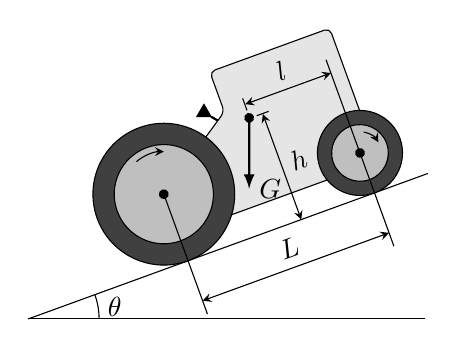
\begin{tikzpicture}[>=stealth,scale=1.8]
  \draw(0,0)--(2.8,0);
  \draw[thin](0.5,0)arc(0:20:0.5)node[midway,right]{$\theta$};
\begin{scope}[rotate=20]
  \draw(0,0)--(3.0,0);
  \filldraw(1.7,0.9)--++(100:0.1)--++(220:0.1)--cycle;
  \draw[thick](1.7,0.9)--++(-50:0.2);
  \draw[fill=lightgray!40,rounded corners=2pt](1.0,0.2)--(2.7,0.2)--(2.7,1.2)--(1.8,1.2)--(1.8,0.9)--(1.2,0.5)--cycle;
  \draw[fill=darkgray](1.2,0.5) circle(0.5);
  \draw[fill=lightgray](1.2,0.5) circle(0.35);
  \draw[fill=darkgray](2.6,0.3) circle(0.3);
  \draw[fill=lightgray](2.6,0.3) circle(0.2);
  \draw[thin](1.2,0.5)--(1.2,-0.4)(2.6,1.0)--(2.6,-0.4);
  \draw[thin,<->](1.2,-0.3)--(2.6,-0.3)node[midway,rotate=20,above]{$L$};
  \draw[thin,|<->](1.95,0.9)--(2.6,0.9)node[midway,rotate=20,above]{$l$};
  \draw[thin,<->|](2.05,0)--(2.05,0.8)node[midway,rotate=20,right]{$h$};
  \draw[thick,-latex](1.95,0.8)--++(250:0.5)node[right]{$G$};
  \fill(1.2,0.5)circle(1pt);
  \fill(2.6,0.3)circle(1pt);
  \fill(1.95,0.8)circle(1pt);
  \draw[thin,->]([shift=(110:0.3cm)]1.2,0.5)arc(110:70:0.3);
  \draw[thin,->]([shift=(60:0.15cm)]2.6,0.3)arc(60:10:0.15);
\end{scope}
\end{tikzpicture}
\end{document}